\documentclass[11pt]{article}
\usepackage{graphicx}
\usepackage{float}
\usepackage{amsmath}
\usepackage{amsfonts}
\usepackage[brazilian]{babel}
\usepackage[utf8]{inputenc}
\usepackage[backend=biber]{biblatex}
\usepackage{csquotes}
\usepackage{docmute}
\usepackage{array}
\usepackage[T1]{fontenc}

\addbibresource{plano_de_pesquisa.bib}

\newcommand{\fromeng}[1]{\footnote{do inglês: \textit{#1}}}
\newcommand{\tit}[1]{\textit{#1}}
\newcommand{\tbf}[1]{\textbf{#1}}
\newcommand{\ttt}[1]{\texttt{#1}}

\newcolumntype{C}[1]{>{\centering\let\newline\\\arraybackslash\hspace{0pt}}m{#1}}

\begin{document}

\begin{titlepage}
	\centering
	{\scshape\Large Projeto de pesquisa\par}
	\vspace{1.5cm}
	{\huge\bfseries Processos atencionais e aprendizado de máquina 
		para sistemas robóticos\par}
	\vspace{1cm}
	{\itshape Aluno: Erik de Godoy Perillo\par}
	{\itshape Orientadora: Esther Luna Colombini\par}
	\vspace{0.5cm}
	\begin{abstract}
		Entender o ambiente ao seu redor é uma tarefa fundamental para 
		o desafio de se obter máquinas autônomas que interagem com o 
		ambiente de forma semelhante à nossa.
		A alta dimensionalidade dos dados captados por sensores usados para 
		este fim é em geral problemática pois muitas vezes há
		redundância e irrelevância de informação. 
		Neste projeto, propomos o uso de processos atencionais em cascata 
		com aprendizado de máquina a fim de se obter um sistema de 
		identificação de classificação de objetos em um dado ambiente
		que seja eficiente, preciso e geral. 
		Por fim, planeja-se implementar uma estrutura que permita o uso das
		técnicas por projetos robóticos em geral em GPUs embarcadas.
	\end{abstract}
	\vfill
	Universidade Estadual de Campinas 
	\vfill
	{\large \today\par}
\end{titlepage}

\newpage

\section{Introdução}
\paragraph{}
Máquinas capazes de realizar tarefas complexas, perigosas ou maçantes são
objeto de interesse e desejo do ser humano há tempos. 
Robôs industriais já dominam os mais variados setores de produção. 
Não apenas parados em linhas de montagem, sistemas atuais podem locomover-se
em regiões uniformes e previsíveis -- como galpões de estoques -- trabalhando
vinte e quatro horas por dia~\cite{warehouse}.
Um desafio ainda em aberto, entretanto, é a concepção de robôs que lidam com 
o imprevisível, reagindo de forma apropriada às mais diversas situações 
e ambientes do mundo real. 

Sistemas que interagem com o ambiente, objetos e pessoas 
com uma variedade de maneiras semelhante à nossa têm o potencial de ser 
incrivelmente benéficas para a sociedade. 
%Esse tipo de robô tem sido tendência ...
Diversos desafios fascinantes estão associados ao processo de concepção de 
máquinas gerais desse tipo. 
Um deles, certamente, é a compreensão. 
Entender o que lhe cerca é fundamental para uma interação complexa com o resto
do mundo. 

Ter ciência de sua relação espacial com outros objetos e 
suas possíveis interações com cada um deles é essencial para a navegação 
de robôs por casas, ruas e até mesmo locais que seriam impossíveis 
para um ser humano estar. 
Essa é uma das tarefas principais que máquinas como carros autônomos, 
robôs caseiros e de resgate devem cumprir bem.
Técnicas que utilizam sensores como câmeras~\cite{vision} e LIDAR~\cite{car} 
têm sido usadas com sucesso para identificação e classificação de entidades 
em um ambiente com o qual o robô interage. 

\subsection{Motivação}
\paragraph{}
Um problema de sensores usados para tarefas mais complexas de navegação
em geral -- como câmera e LIDAR  --
é que seus volumes de dados podem ser demasiadamente grandes. 
Em um momento qualquer, é improvável que 
toda a informação provida de um sensor seja necessária. 
Lidar com todo o conjunto de dados para depois determinar qual parte é 
relevante pode ser uma tarefa muito custosa computacionalmente. 
Isso é especialmente crítico para sistemas robóticos que precisam de respostas
rápidas para interar com o ambiente em que estão inseridos. 

Além disso, o \tit{hardware} utilizado em robôs autônomos tem sido por muitos 
anos limitado pelas restrições de em geral ter de ser embarcado e compacto.
Avanços recentes têm mudado isso, entretanto. 
Além do aumento da eficiência e diminuição do tamanho de CPUs impulsionado
pelo mercado \tit{mobile}, esforços têm sido feitos para a concepção de 
computadores com processadores gráficos (GPUs) embarcados. 
A \tit{NVIDIA} lançou recentemente os modelos 
\tit{Jetson TK1} e \tit{Jetson TX1}~\cite{jetson}, que são computadores 
completos com GPUs poderosas e energeticamente eficientes neles inclusas, 
desenvolvidos especialmente para serem embarcados em projetos móveis.
O uso de GPUs em robótica abre a possibilidade do uso de técnicas mais 
sofisticadas e computacionalmente caras que até então não podiam ser exploradas.
Sua natureza paralela permite um grande benefício de operações que podem ser
divididas em subproblemas e realizados ao mesmo tempo. 
Esse é o caso de diversas tarefas como processamento de sinais e técnicas 
de aprendizado de máquina~\cite{gpu}, por exemplo. 

\subsection{Processos atencionais e aprendizado de máquina}
\paragraph{}
O fato de sensores darem uma quantidade muito grande de informação que nem 
sempre é necessária motiva uma abordagem inspirada no ser humano.
Não damos foco a todas as conversas que escutamos ou em tudo que vemos, mas sim 
apenas na parte que nos convém. 
Técnicas que fazem uso de processos atencionais têm sido usadas para a 
segmentação de áreas de relevância na percepção e entendimento do 
ambiente com sucesso~\cite{bio}~\cite{esther}.
Com essas abordagens, pode-se filtrar muito do que seriam dados irrelevantes ou
redundantes, aumentando consideravelmente a eficiência computacional dessas
técnicas.

Não só o foco é necessário: em ambientes dos mais variados é necessário, além
de identificar, classificar entidades a fim de interagir com elas de forma
apropriada. 
O aprendizado de máquina tem sido uma área de grande sucesso nessa tarefa.
Diversas técnicas podem ser utilizadas, como \tit{SVMs}~\cite{svm} 
e redes neurais~\cite{nn} a fim de se classificar entidades em geral com 
alta taxa de acertos. 

O que se busca, então, é uma mescla dessas duas técnicas: o uso dos processos
atencionais em um estágio inicial de processamento pode atuar como um filtro
na informação, passando adiante somente o que é relevante para o estágio de
classificação com uso de técnicas robustas de aprendizado de máquina. 
O que se espera é que tal abordagem possibilite uma percepção eficiente, geral
e complexa do ambiente para sistemas autônomos, o que os possibilitaria 
realizar tarefas mais sofisticadas e traria benefícios objetivos para
a área da percepção em robótica.

\section{Objetivos}
\paragraph{}
Os objetivos deste trabalho são:
\begin{itemize}
	\item Obter técnicas que permitam a percepção em ambientes
		diversos para a navegação de sistemas robóticos autônomos por meio 
		do uso de processos atencionais e aprendizado de máquina.
	\item Realizar uma avaliação de efetividade e eficiência de nossa abordagem
		e compará-la com outras técnicas utilizadas atualmente.
	\item Construção de uma plataforma para uso em GPUs embarcadas com 
		ferramentas que permitam o uso de nossa técnica desenvolvida para
		aplicações variadas de robótica.
\end{itemize}

\section{Materiais e Métodos}
\subsection{Caso de uso}
\paragraph{}
O desafio \tit{Trekking}~\cite{trekking_regras} é uma categoria da série de 
competições de robótica realizada pela \tit{Robocore}~\cite{robocore}. 
Nessa categoria, o robô deve completar um percurso em 
um campo de futebol passando por diversas bases em uma ordem pré-definida.
Em uma certa região do campo, há obstáculos dos quais o robô deve desviar.
O percurso deve ser feito no menor tempo possível.

\begin{figure}[H]
  		\centering
    	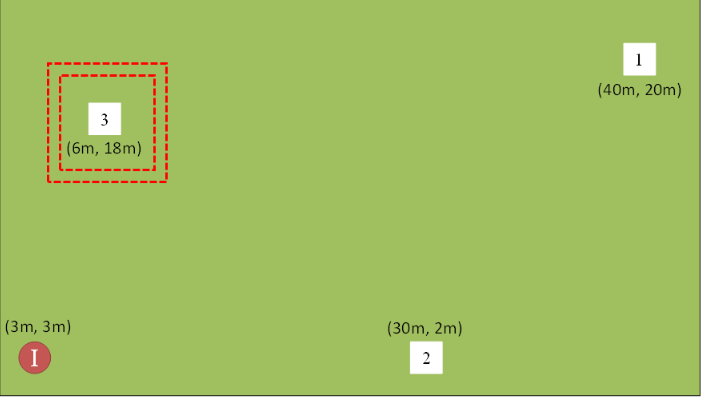
\includegraphics[width=0.6\textwidth]{imgs/trekking_campo.png}
		\caption[9pt]{O ambiente de locomoção do robô na categoria Trekking}
\end{figure}

A \emph{Equipe Phoenix de Robótica da Unicamp}~\cite{phoenix} 
é formada por estudantes de graduação de diversos cursos de 
Engenharia e Computação da Universidade Estadual de Campinas. 
Na equipe, desenvolvem-se variados projetos de robótica,
com foco principal em robôs para competir nas categorias das competições da
\tit{Robocore}.  
A equipe desenvolve atualmente um robô para participar na categoria 
\tit{Trekking}, nomeado \tit{Projeto Piranha}. 
O robô consiste em um carro elétrico com tração nas quatro rodas e 
locomoção por motores \tit{brushless}.
O motor é controlado por meio de um conjunto da \tit{NXP} composto da placa
\ttt{FRDM-K64F} e da placa \ttt{FRDM-STBC-AGM01}~\cite{nxp}, que contém 
diversos sensores inerciais como magnetômetro, giroscópio e acelerômetro.
Há também um kit de desenvolvimento com GPU embarcada \tit{NVIDIA Jetson TX1}. 
A \tit{Jetson TX1} possui um processador \tit{ARM Quad-Core Cortex-A57},
4GB de memória \tit{RAM} e uma GPU \tit{NVIDIA Maxwell} com 256 núcleos de
processamento~\cite{tx1}. 
Seu sistema operacional é o Ubuntu com \tit{kernel Linux}.
Duas câmeras \tit{Logitech C270} são os sensores
principais usados pela \tit{Jetson TX1} para a ambientação do robô no campo.

\begin{figure}[H]
  		\centering
    	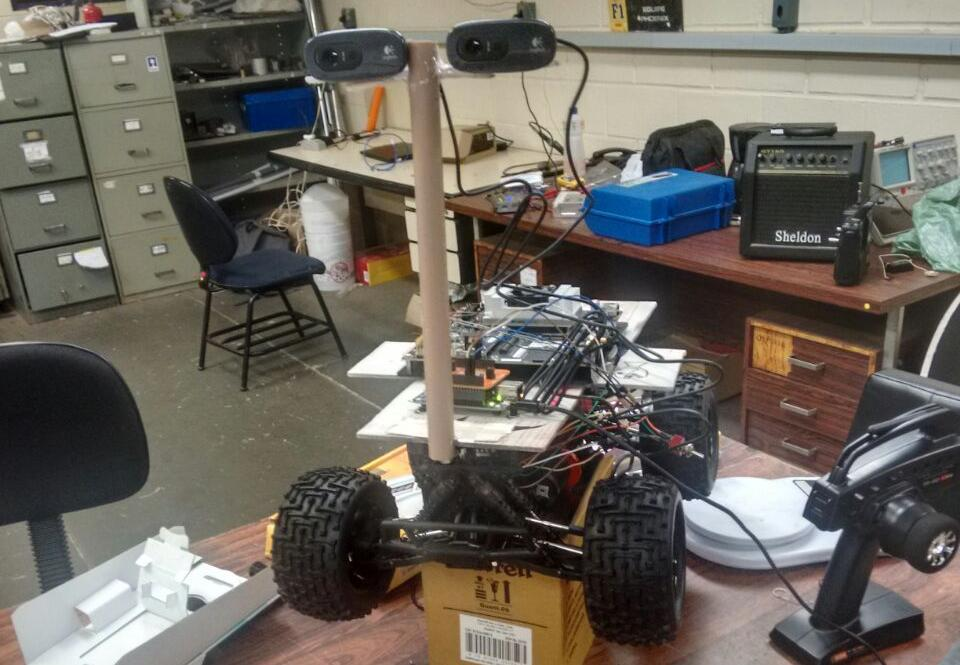
\includegraphics[width=0.6\textwidth]{imgs/piranha.jpg}
		\caption[9pt]{O robô do projeto Piranha}
\end{figure}

A pesquisa usará o robô \tit{Piranha} como caso de uso para
avaliação da abordagem a ser desenvolvida, com o uso da \tit{Jetson TX1} 
como plataforma para implementação das técnicas.
O robô usa a câmera como principal sensor.
Assim, a pesquisa foca em imagens como o sinal a ser processado e analisado. 

A ideia é aplicar as técnicas a se obter para o reconhecimento
de entidades na imagem, como terreno o qual o robô pode andar, obstáculos do
qual deve desviar e bases às quais deve-se chegar.
Soluções em processos atencionais serão desenvolvidas separadamente do
estágio de classificação de objetos com aprendizado de máquina. 
Após isso, a união dos dois será feita.

\subsection{Avaliação da abordagem proposta}
\paragraph{}
Será feita uma comparação com três técnicas diferentes: 
\begin{enumerate}
	\item Uma abordagem específica é utilizada.  
		Um simples \tit{threshold} de cor pode ser capaz de identificar objetos
		imagem e classificá-los dado que diferentes classes de objetos têm
		diferentes cores.
	\item Aprendizado de máquina puro para reconhecimento de objetos.
		Nessa abordagem, será dado foco igual a toda a informação. 
		Assim, todo o conjunto deverá ser analisado pelos algoritmos.
	\item Processos atencionais são utilizados em um estágio anterior ao de 
		classificação com aprendizado de máquina, com a intenção de selecionar
		subconjuntos de toda informação dada pelo sensor que tenham maior 
		relevância para serem analizados no estágio de classificação.
\end{enumerate}

Com essa comparação, espera-se avaliar cada técnica pelos seguintes critérios:
\begin{itemize}
	\item Desempenho: o custo computacional da técnica.
	\item Eficiência: quão corretamente a técnica identifica e classifica
		as entidades de interesse.
	\item Generalidade: possibilidade da técnica ser utilizadas em outros 
		cenários.
\end{itemize}

\subsection{Construção de plataforma para navegação usando GPUs}
\paragraph{}
Com as técnicas obtidas pelo projeto, espera-se construir uma plataforma
de uso geral para robôs autônomos que usem GPUs embarcadas.
\tit{frameworks} de aprendizado de máquina serão estudados para se decidir
quais usar. 
Toda biblioteca será escolhida de forma que se possa utilizar o processamento
da GPU.
Por meio da linguagem de programação \tit{C++} juntamente com \tit{Python},  
um ambiente de treinamento e rotinas de classificação para uso em imagens
será desenvolvido.

\section{Cronograma}
\paragraph{}
\begin{table}[H]
\setlength{\tabcolsep}{.16667em}
\begin{tabular}{|C{5cm}|c|c|c|c|c|c|c|c|c|c|c|c|}
	\hline
	Tarefa/mês & Jul & Ago & Set & Out & Nov & Dez & Jan & Fev & Mar & Abr & Mai & 
	Jun \\
	\hline
	Revisão Bibliográfica & x & & & & & & & & & & & \\
	\hline
	Modelagem de processos atencionais & & x & x & & & & & & & & & \\
	\hline
	Modelagem aprendizado de máquina & & & x & x & & & & & & & & \\
	\hline
	Coleta de imagens para treinamento & & & & & x & & & & & & & \\
	\hline
	Integração dos sistemas & & & & & & x & & & & & & \\
	\hline
	Implementação de técnicas & & & & & & & x & x & & & & \\
	\hline
	Testes comparativos & & & & & & &  & & x & & & \\
	\hline
	Construção de plataforma para GPU & & & & & & & & & & x & x & \\
	\hline
	Relatório final & & & & & & & & & & & & x \\
	\hline
\end{tabular}
\end{table}

\printbibliography

\end{document}
